% PACKAGES INCLUDED HERE 
% DO NOT NEED TO CHANGE
\documentclass[conference]{IEEEtran}
%\IEEEoverridecommandlockouts
% The preceding line is only needed to identify funding in the first footnote. If that is unneeded, please comment it out.
\usepackage{listings}
\usepackage{csquotes}
\usepackage{float}
\usepackage[caption=false]{subfig}
\usepackage{cite}
\usepackage{amsmath,amssymb,amsfonts}
\usepackage{algorithmic}
\usepackage{graphicx}
\usepackage{textcomp}
\usepackage{hyperref}
\usepackage{url}
\usepackage{amsmath}
\def\BibTeX{{\rm B\kern-.05em{\sc i\kern-.025em b}\kern-.08em
    T\kern-.1667em\lower.7ex\hbox{E}\kern-.125emX}}
\begin{document}

% TITLE GOES HERE

\title{Predicting Pseudo Random Values Using Convolutional Neural Networks\\}

\IEEEspecialpapernotice{\\Middle Tennessee State University\\1301 East Main Street
Murfreesboro, TN 37132-0001\\Department of Computer Science\\~\\}


% AUTHOR NAMES GOES HERE
\author{
\IEEEauthorblockN{1\textsuperscript{st} Spencer Arnold}
sra4d@mtmail.mtsu.edu \\
sa.education@outlook.com\\[0.4cm]  %<------- Extra vertical space
\IEEEauthorblockN{4\textsuperscript{th} Matthew Hawks}
mdh7r@mtmail.mtsu.edu \\
\and
\IEEEauthorblockN{2\textsuperscript{nd} Abdinajib Ali}
aaa2ak@mtmail.mtsu.edu\\
hanut.ali96@gmail.com\\[0.4cm]  %<------- Extra vertical space
\IEEEauthorblockN{5\textsuperscript{th} Ryan Hines}
rch5b@mtmail.mtsu.edu \\
\and
\IEEEauthorblockN{3\textsuperscript{rd} Jacob Anderson}
jaa5v@mtmail.mtsu.edu\\[0.8cm]  %<------- Extra vertical space
\IEEEauthorblockN{6\textsuperscript{th} Tae Kweon}
thk2e@mtmail.mtsu.edu \\
}
\maketitle

% ABSTRACT 
\begin{abstract}
Pseudo-Random number generators (PRNG) are a cornerstone if not the foundation for cryptography. The quality of generated pseudo-random numbers (PRN) can usually determine the "cryptographic strength" of a given system. As history shows us, there have been numerous attempts to create PRNGs that decrease the general predictability and correlation of each subsequent value produced. We introduce a novel approach to predicting sequences of given PRNGs by proposing the use of deep convolutional networks (CNN) in a regression-based supervised learning process.
We also provide an experimental framework for the latter and, in addition to building off of existing prediction models, we demonstrate that the cryptographic strength of each consecutive PRNG increases, while prediction success rates (even with learning) are generally less effective. At the core, this is based upon the nature of the increasing importance of stronger PRNGs across industries.
\end{abstract}

% KEYWORDS
\begin{IEEEkeywords}
pseudo random number (PRN), pseudo random number generator (PRNG), convolutional neural networks (CNN), neural cryptography.
\end{IEEEkeywords}

% INTRODUCTION SECTION
\section{Introduction}
Society relies on Pseudo-random numbers for a multitude of reasons. Whether the use cases fall in Information Security or, more broadly, modeling and simulation, we think it is important to not only push the boundary for the modern pseudo-random number directly but to also analyze the history of pseudo randomness to aide in that effort. Whether true randomness is an inhibition of the human perception or not, there is a clear need to push the modern pseudo-random number closer to converging on perceived "true" randomness.
Our main aim was to train a predictive neural net to predict the values of different PRNGs and come to generalized conclusions about the development of PRNGs with respect to time, in addition to any PRN correlations we uncover.

We approached this goal by implementing five PRNGs:
\begin{itemize}
  \item Middle-square method (1946)
  \item Linear congruential generator (1958)
  \item Lagged Fibonacci (1965)
  \item Park-Miller (1988)
  \item Mersenne Twister (1998)
\end{itemize}

These PRNGs will be looked at in depth in the methods section, but we mainly chose these five because they represent key points of progression in the developement of stronger PRNGs chronologically. Although five were chosen, the door is open to test other PRNGs in future research.

Before conducting the research, we formed the following hypotheses:
\begin{enumerate}
    \item We predict there will be a positive trend over time on the cryptographic strength of each subsequent PRNG, given the nature of the increasing importance of stronger PRNGs.
    \item We also predict that, as we get into cryptographically stronger generation methods, our prediction success rates (even with learning) will be less effective.
    \item We expect to uncover correlations in PRNs based on each individual generator and aim to extract more generalized correlations between generators themselves.
\end{enumerate}

% BACKGROUND SECTION
\section{Background}
PRNGs are generally deterministic algorithms that take in an input seed to generate PRNs that may or may not be tractable using statistical means. In this research, we use convolutional neural networks to try to predict the next set of random numbers generated from a PRNG. 
Typically, convolutional neural nets (CNNs) are used to tackle image classification problems; however, their design, stemming from the architecture of an underlying multi-layer perceptron, allows localized pattern detection that is extremely powerful in gaining insight from potentially noisy data, as in common cases of signal processing.\cite{Markell94}
"CNNs exploit spatial locality by enforcing a local connectivity pattern between neurons of adjacent layers. The architecture thus ensures that the learned "filters" produce the strongest response to a spatially local input pattern." \cite{CNN}
This is useful in problems where sequential analysis (like in time series problems) is prevalent. Oftentimes, CNNs are viewed as introductory ways of image classification without many other applications. When thinking of pixel data as an enumerated sequence of numbers, one can start to uncover the application of CNNs in other areas, like building a regression model for sequences of pseudo-random number data.
In the following sections, we will discuss just that.

% METHODS SECTION
\section{Methods}
\subsection{Seeding Method}
We went with a seed generation method that allowed a way to introduce some minor level of entropy to avoid letting the neural network aimlessly swim through the entropy of a strong seed, instead of gaining stochastic insight on the data from the PRNG.

The seed generation method we chose derives from the concept of using the system time as an element for seed generation. The specific implementation we chose took inspiration from Microsoft's .NET system.datetime.ticks property. \cite{msoftdocs} We chose to single out this method due to its documentation and unique simplicity. In general, system time is widely used as a parameter for modern seed generation methods. 

To put it more trivially: "a pseudo-random number generator is a deterministic algorithm that, given an initial number (called a seed), generates a sequence of numbers that adequately satisfy statistical randomness tests. Since the algorithm is deterministic, the algorithm will always generate the exact same sequence of numbers if it's initialized with the same seed. That's why system time (something that changes all the time) is usually used as the seed for random number generators." \cite{pseudoquote}

According to the Microsoft documentation, "A single tick represents one hundred nanoseconds or one ten-millionth of a second. There are 10,000 ticks in a millisecond, or 10 million ticks in a second. The value of this property represents the number of 100-nanosecond intervals that have elapsed since 12:00:00 midnight, January 1, 0001 in the Gregorian calendar." \cite{msoftdocs}

We used a fairly similar Python port, as seen in Figure ~\ref{fig:Default Seeding Method}

\begin{figure}[H]
\centering
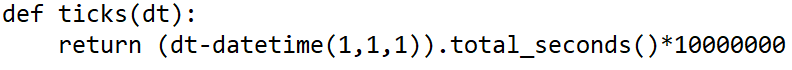
\includegraphics[width=1\linewidth]{./Images/Ticks.png}
\caption{Default Seeding Method}
\label{fig:Default Seeding Method}
\end{figure}

This python port of Microsoft's tick method can be attributed to "mhawke" on StackOverflow. \cite{tickport} The author had some noteworthy comments about this implementation, namely some porting side effects:
\begin{enumerate}
    \item UTC times are assumed.
    \item The resolution of the DateTime object is given by DateTime.resolution, which is DateTime.timedelta(0, 0, 1) or microsecond resolution (1e-06 seconds). CSharp Ticks are purported to be 1e-07 seconds.
\end{enumerate}

For experimental needs, we made additional changes to the implementation:
\begin{enumerate}
    \item Changing start time from January 1, 0001 to January 1, 1970, which effectively reduced the length of the seed for experimental purposes.
    \item Slicing the last 6 digits of the ticks result to acquire more digit variation for frequent invocation.
\end{enumerate}

The final modified method allows enough spread between frequently retrieved ticks, where we are assuming reasonable pseudo-unpredictability. This serves as a simplistic but constantly changing control mechanism for being able to seed PRNGs and test experimental outcomes. While not the most cryptographically strong, we needed a way to have some controlled aspect of seed generation to feed into generators of varying cryptographic complexity (to have some baseline of comparison).

The original idea was to feed each PRNG different seeds from the same seed generator; however, many PRNG algorithms impose strict seed requirements to pass tests of randomness. Out of the five PRNG methods we implemented, Lagged Fibonacci was the only one that had special seed requirements, so we created a separate seed generator based on the same fundamental ticks generation method, but modified it to meet the restrictions. Other PRNGs not implemented in this research that impose seed restrictions include Wichmann-Hill (which accepts three different seeds) and Maximally Periodic Reciprocals (which requires a Sophie Prime), among others.

You might ask: won't different seed generators introduce flaws or bias in the experiment? Well, it depends on what you are testing. In our case, we are strictly testing the "complexity" of the generator itself, so supplying a seed that is not blatantly predictable but also not unpredictable was sufficient. Our goal was to allow the characteristics of the generator to be exposed, for we were cracking the "complexity" of the generation algorithm, not the complexity of an arbitrary seed.

\subsection{PRNG Implementations}
As outlined in the introduction, we chose five PRNG methods by year of invention. Choosing five PRNGs allowed us to focus on implementations, while leaving future research opportunities open for others we did not cover. This sub-section highlights descriptions of the experimental role PRNGs played in our research and descriptions/notes we made about each PRNG implementation we created.

The call definition of any given PRNG function is as follows:
\begin{lstlisting}
PRNGfunc(seed, n) 
\end{lstlisting}

This is so we can experimentally automate the calling of each PRNG without getting too complex.
The given PRNG function should return a list of n generated numbers using the generation method.
All other parameters outside of the seed and n are default values.

For example, if the call was PRNG(seed, 10),
it might return something like
[3,5,10,1,31,17,2,4,6,7]

We control parsing the n-length list and handling seeds externally. 
This plays logically with separation of concerns for our usecase.

While python generators can be useful iterating over previously generated iterables,
we did not want to clutter our experimental execution code, so we stuck to a classical
internal handling of all iterations.

Below are short descriptions and non-inclusive general notes of each PRNG and any implementation notes made during the developement process.


\noindent\textbf{Middle Square}:
\begin{itemize}
    \item "To generate a sequence of n-digit pseudorandom numbers, an n-digit starting value is created and squared, producing a 2n-digit number. If the result has fewer than 2n digits, leading zeroes are added to compensate. The middle n digits of the result would be the next number in the sequence, and returned as the result. This process is then repeated to generate more numbers." \cite{MiddleSquare}
\end{itemize}
Notes:
\begin{itemize}
    \item Generally the value of the seed has to be even, but can be padded with leading zeros.
    \item If the middle n digits are all zeroes, the generator then outputs zeroes indefinitely. If the first half of a number in the sequence is zeroes, the subsequent numbers eventually converges to zero.
\end{itemize}


\noindent\textbf{Linear Congruential}:
\begin{itemize}
    \item A linear congruential generator is a PRNG that represents an "additive  congruential  method", with foundations in improving upon "unsatisfactory" tests with entropy in fibonacci sequences. \cite{10.1145/321008.321019}
\end{itemize}
Notes:
\begin{itemize}
    \item The generator is not sensitive to the choice of c, 
as long as it is relatively prime to the modulus 
(e.g. if m is a power of 2, then c must be odd), 
so the value c=1 is commonly chosen.
    \item If c = 0, the generator is often called a multiplicative
congruential generator (MCG), or Lehmer RNG (which is used for our implementation). If c ≠ 0, the
method is called a mixed congruential generator.
    \item Parameters were chosen based on $2^32$ numbers in table 2 of the article "Tables of linear congruential generators of different sizes and good lattice structure." \cite{LEcuyer1999TablesOL}
\end{itemize}


\noindent\textbf{Lagged Fibonacci}:
\begin{itemize}
    \item The Lagged Fibonacci PRNG is a generalization of the Fibonacci Sequence \cite{lucas1891calcul}, where the sequence is generated based off a seed and the sum of the last two values is the PRN (which is also serves as the next seed).
\end{itemize}
Notes:
\begin{itemize}
    \item It is refered to a "lagged" generator, because "j" and "k" lag behind the generated pseudorandom value. 
    \item Our implementation is called a "two-tap" generator, in that you are using 2 values in the sequence 
to generate the pseudorandom number. However, note that a two-tap generator has some problems with 
randomness tests, such as the Birthday Spacings. Creating a "three-tap" generator could
addresses this problem.
\end{itemize}


\noindent\textbf{Park Miller}:
\begin{itemize}
    \item Park Miller (also known as Lehmer) can be viewed as a particular case of the Lemher PRNG, which is a particular case of the linear congruential PRNG, where c=0 and particular parameters are specified.
\end{itemize}
Notes:
\begin{itemize}
    \item "In 1988, Park and Miller \cite{10.1145/63039.63042}, suggested a Lehmer RNG with particular parameters m = 231 − 1 = 2,147,483,647 (a Mersenne prime M31) and a = 75 = 16,807 (a primitive root modulo M31), now known as MINSTD." \cite{ParkMiller}
\end{itemize}


\noindent\textbf{Mersenne Twister}:
\begin{itemize}
    \item "The Mersenne Twister algorithm is based on a matrix linear recurrence over a finite binary field" \cite{10.1145/146382.146383}
\end{itemize}
Notes:
\begin{itemize}
    \item This PRNG is similar to a common LFSR. Its MT19937 implementation is probably the most commonly used modern PRNG. 
    \item It is also the default generator in the Python language starting from version 2.3. 
    \item For our implementation, we used numpy's version of the Mersenne Twister.
\end{itemize}


\subsection{Experimental Setup}


The following is a vastly informal mathematical representation of our experimental model, using a loose coupling of TLA+ notation and some set-builder theory. Further explanations and graphics will follow to aid in the interpretation of the design of the experimental setup.

\begin{displayquote}
Let $n$ be any arbitrary natural number such that $\{n \in \mathbb{N}\}$.
Let $E$ represent the experiment definition.
Let $seed$ be a function such that when called will return a seed.
Given $k$ and $S_n$, let $prng$ be a function such that when called will return a set of pseudo random numbers,
dervied from an initial seed $S_n$ and a given algorithm, where the length of the set is $k$.
\end{displayquote}

\begin{figure}[H]
\centering
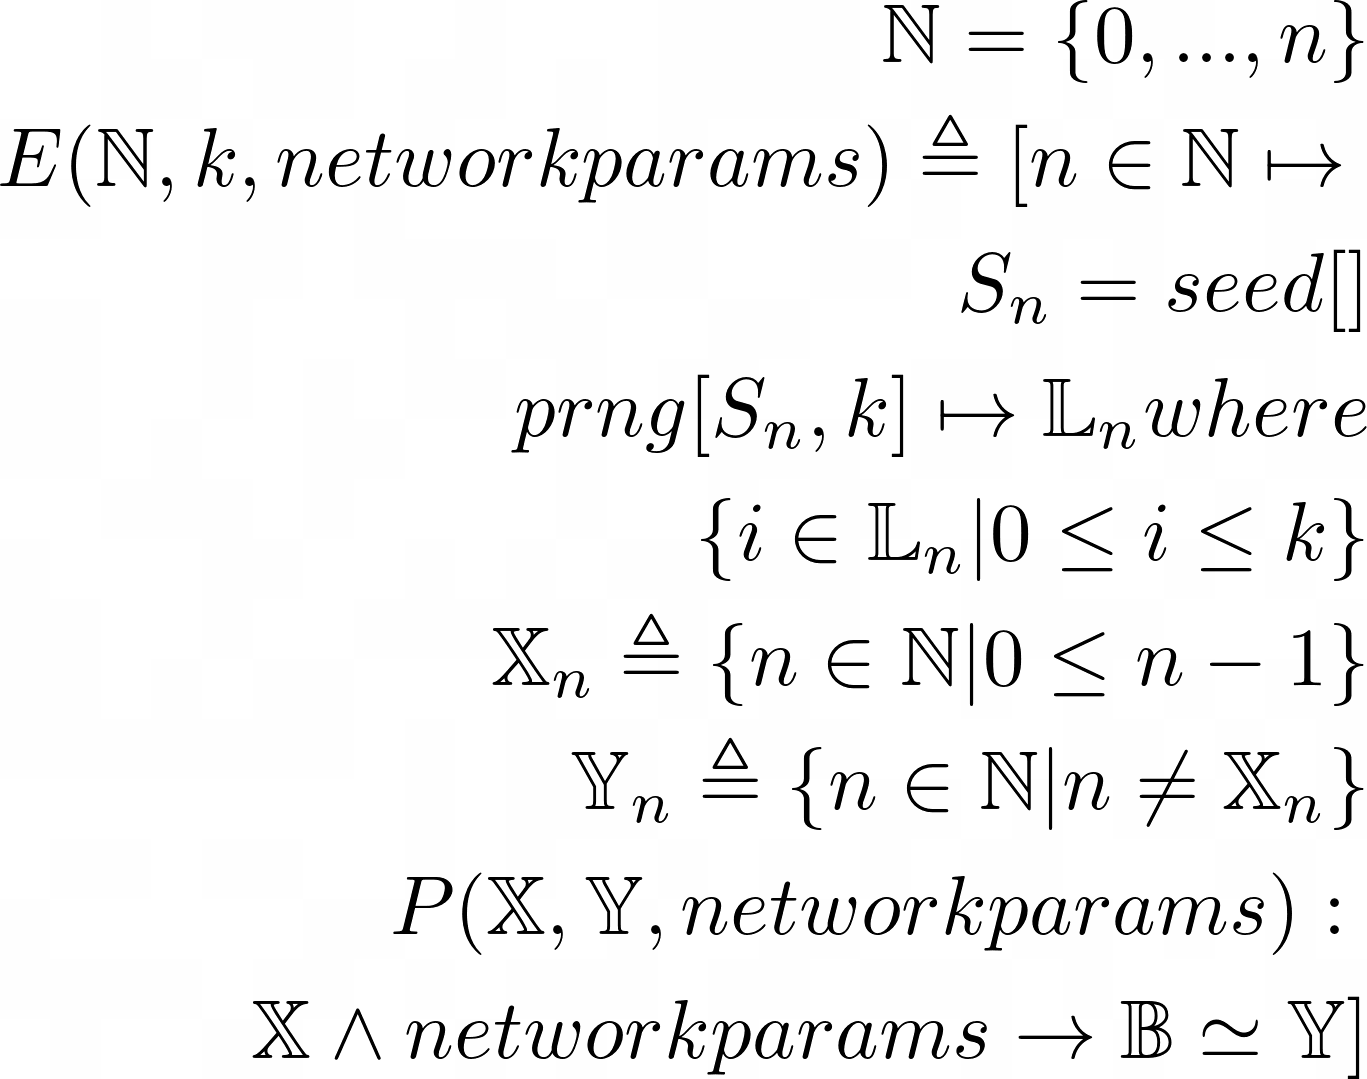
\includegraphics[width=.5\linewidth]{./Images/ModelNotated.png}
\caption{Notated Experiment Model}
\label{fig:Notated Experiment Model}
\end{figure}


Given an enumerated set, $\mathbb{N}$,
where $prng$ is the chosen PRNG, $S_n$ is $n$th seed in the iteration, and $k$ is the length of the desired output vector ($\mathbb{L}_n$) of $prng$,
$\mathbb{X}_n$ represents an enumerated set containing $n$ sets of $k-1$ values generated from a PRNG ($prng$) and each $\mathbb{X}_n$ set is derived from a different seed. $\mathbb{Y}_n$ represents a set containing $n$ sets of $k$th values with a direct mapping to each $\mathbb{X}_n$ such that $\mathbb{X}_n \mapsto \mathbb{Y}_n$. $P$ a predictor function that represents a convolutional neural network, which takes in $\mathbb{X}_n$ and $\mathbb{Y}_n$, yields a new set $\mathbb{B}_n$ implied from $\mathbb{X}_n$, where the model trains $\mathbb{B}_n$ to be similar or equal to $\mathbb{Y}_n$ based on back-propagation due to previous predictions, thus using supervised learning to build a regression model.

For a simplified graphical representation of the latter description, please reference the predictive model in Figure~\ref{fig:Predictive Model}, the simplified experimental model in Figure~\ref{fig:Simplified Experimental Model}, and the granular view of the experimental model in Figure~\ref{fig:Granular Experimental Model}.


\begin{figure}[H]
\centering
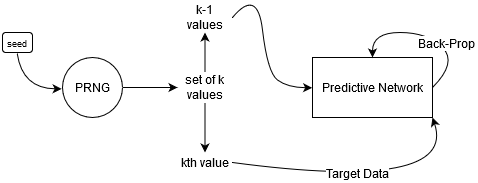
\includegraphics[width=1\linewidth]{./Images/SimpleModel.png}
\caption{Simplified Experimental Model}
\label{fig:Simplified Experimental Model}
\end{figure}

Referencing Figure~\ref{fig:Simplified Experimental Model}, which is a visualization of what a 1-dimensional architecture of our experiment might entail, the predictive neural net as visualized in Figure~\ref{fig:Predictive Model} is fed outputs of a specific PRNG, which will attempt to predict a kth value, based on previous k-1 values in a particular set of input data, where each set is generated based off of a single unique seed. After being trained on, ideally thousands of sets, the predictive network will form a better stochastic "understanding" of how the PRNG works underneath, thus being able to more accurately predict numbers generated from that PRNG in the future (i.e., a supervised regression model). The backpropagation will flow through the predictive network to achieve the adversarial nature of a traditional GAN setup, but in reality, we won't be using a generative network, but rather a PRNG algorithm, so the generative part of our setup won't be defensive.


\begin{figure}[H]
\centering
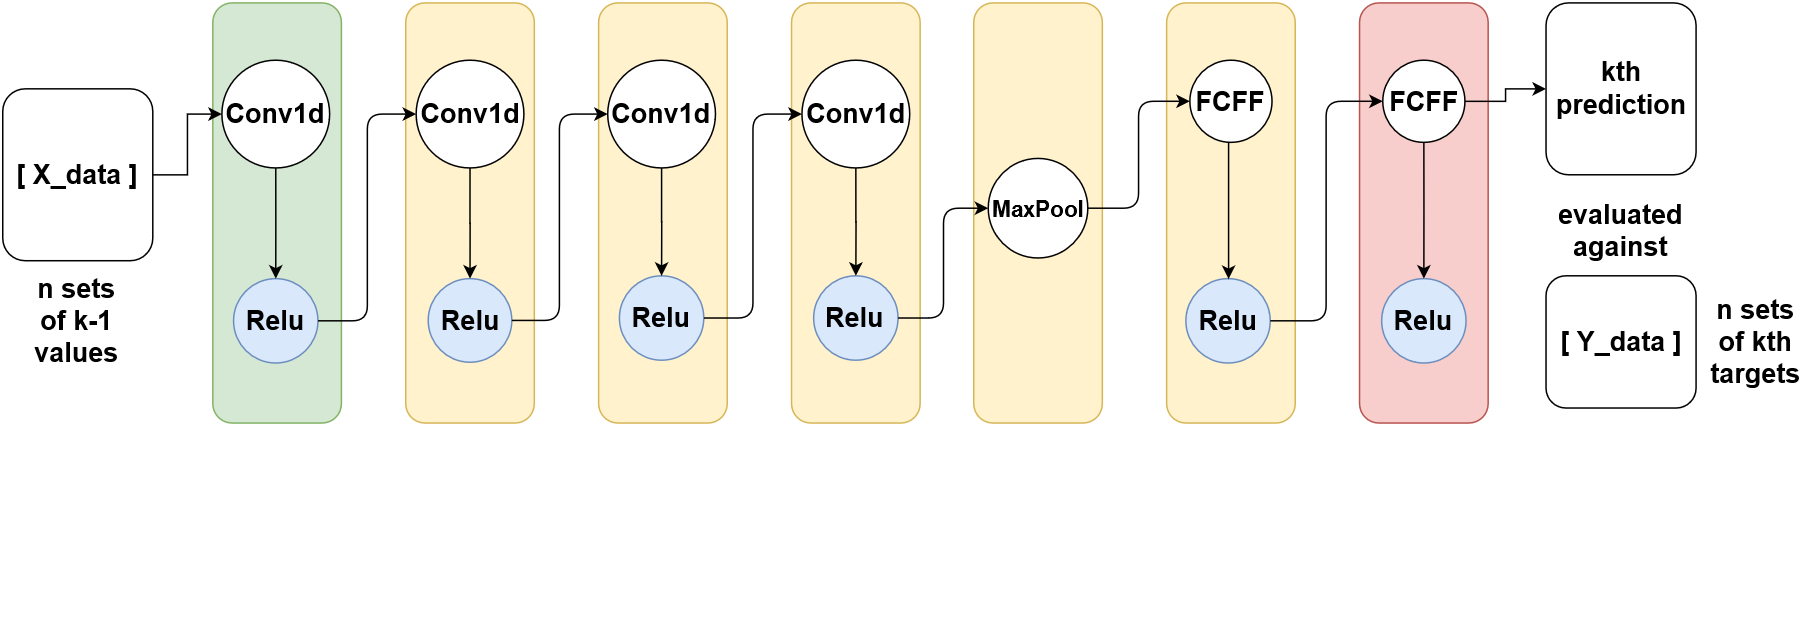
\includegraphics[width=1\linewidth]{./Images/PredictiveModel.png}
\caption{Predictive Model}
\label{fig:Predictive Model}
\end{figure}

Referencing Figure~\ref{fig:Predictive Model}, which is a visualization of the layer stack we used for the predictive network in each trial of the experiment, it "consists of four stacked convolutional layers, each with 4 filters, kernel size 2, and stride 1, followed by a max-pooling layer and two FCFF layers with 4 and 1 units, respectively. The stack of convolutional layers allow the network to discover complex patterns in the input." \cite{debernardi2018pseudo} We used the existing design of research in a similar area at the aforementioned quote. We were able to adapt their discriminative model to fit the needs of our predictive model. The main difference in our model is that we implemented Relus instead of leaky-relus. The meaning of our input and output was also inherently different. View the granular model Figure~\ref{fig:Granular Experimental Model} for more detail on how the input data sets were generated.

\begin{figure}[H]
\centering
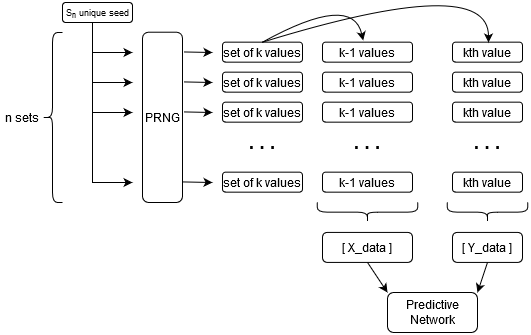
\includegraphics[width=1\linewidth]{./Images/GranularModel.png}
\caption{Granular Experimental Model}
\label{fig:Granular Experimental Model}
\end{figure}

Referencing Figure~\ref{fig:Granular Experimental Model}, which is a granular visualization of our experiment, representing the multi-dimensionality in the generation and aggregation of our data. Note that this is the same general process as illustrated in Figure~\ref{fig:Predictive Model}. The splitting occurs with the data set that is output from the PRNG, which is of k-length, where k-1 values and kth values get split into separate vectors. Note that the data generation and aggregation process is repeated twice: once to produce the training data and once to produce the testing data. Given the fact that we are using PRNs as our training and testing data, this allows us the flexibility to generate thousands of data sets, whereas in most problems concerning neural networks, training and testing data sets are pre-validated and oftentimes this data is limited. Given the circumstance, we could generate an arbitrary amount of training and testing data, given that our PRNG implementation is mathematically sound and algorithmically robust.

\subsection{Experimental Execution}
For the execution of the experiment, we invoked an experimental process and predictive model as described in the last section. We then loaded each PRNG individually and executed the experiment with the following parameters for training: 
\begin{itemize}
\item Number of sets: 1000
\item Length of each set (where each set gets a new seed): 2000
\item batch size: 15
\item Number of epochs: 30
\item Validation split: 0.3
\item Optimization method: nadam
\item Learning rate: 0.001
\item Loss method: mean absolute error
\end{itemize}

After training, we had five separate trained prediction models corresponding to each PRNG. We then tested our models with the testing data and produced correlation coefficients to track how well our models represented new test data from each PRNG.

% RESULTS SECTION
\section{Results}
The following are the regression and loss plots resulting from the testing of each predictive model.
\begin{figure}[H]
\centering
\subfloat[Subfigure 1 list of figures text][Testing Regression Plot]{
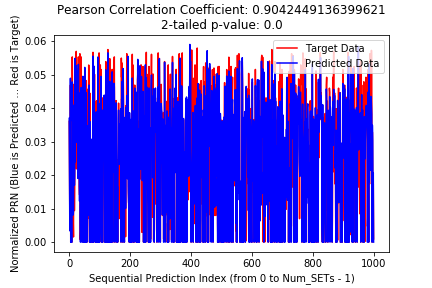
\includegraphics[width=0.4\linewidth]{./Images/Middle_Square_Reg.png}
\label{fig:MS_A}}
\qquad
\subfloat[Subfigure 2 list of figures text][Training Loss Plot]{
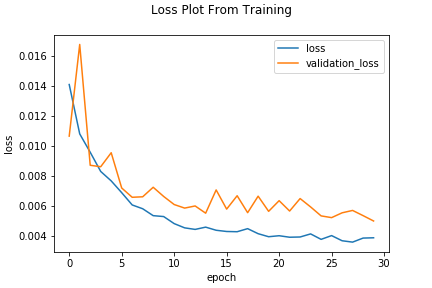
\includegraphics[width=0.4\linewidth]{./Images/Middle_Square_Loss.png}
\label{fig:MS_B}}
\caption{Middle Square Results}
\label{fig:MS}
\end{figure}

Referencing Figure~\ref{fig:MS}, our predictive model did quite well; representing about 90% of the variability in the data from the middle square PRNG.

\begin{figure}[H]
\centering
\subfloat[Subfigure 1 list of figures text][Testing Regression Plot]{
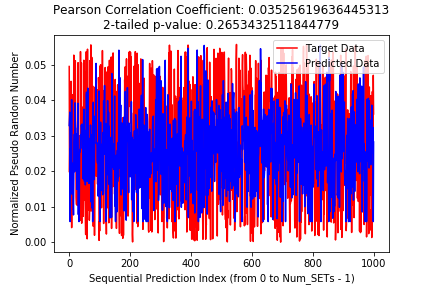
\includegraphics[width=0.4\linewidth]{./Images/Linear_Cong_Reg.png}
\label{fig:LCG_A}}
\qquad
\subfloat[Subfigure 2 list of figures text][Training Loss Plot]{
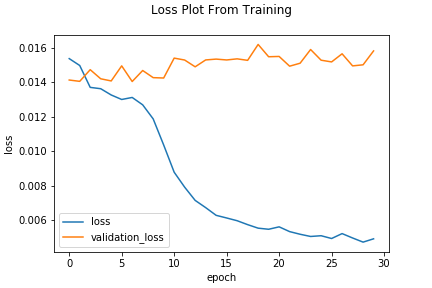
\includegraphics[width=0.4\linewidth]{./Images/Linear_Cong_Loss.png}
\label{fig:LCG_B}}
\caption{Linear Congruential Results}
\label{fig:LCG}
\end{figure}

Referencing Figure~\ref{fig:LCG}, our predictive model did not do well; representing about 3.5% of the variability in the data from the linear congruential PRNG. Note that with a 2-tailed p-value of 0.26, there is an indication of weak evidence for a strong model, so we can not be conclusive. We believe that increasing the quantity of training data would aide in making this a stronger model with a higher correlation coefficient and lower p-value, in addition to more training time.

\begin{figure}[H]
\centering
\subfloat[Subfigure 1 list of figures text][Testing Regression Plot]{
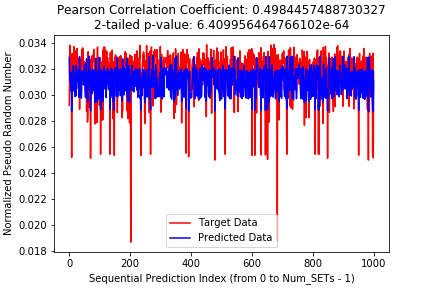
\includegraphics[width=0.4\linewidth]{./Images/Lagged_Fib_Reg.png}
\label{fig:LF_A}}
\qquad
\subfloat[Subfigure 2 list of figures text][Training Loss Plot]{
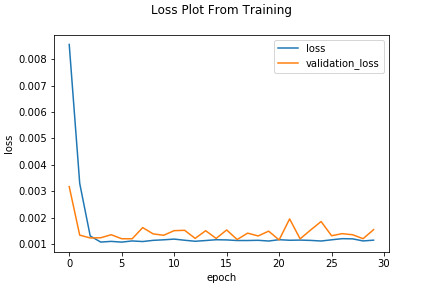
\includegraphics[width=0.4\linewidth]{./Images/Lagged_Fib_Loss.png}
\label{fig:LF_B}}
\caption{Lagged Fibonacci Results}
\label{fig:LF}
\end{figure}

Referencing Figure~\ref{fig:LF}, our predictive model did not do well; representing about 49% of the variability in the data from the lagged fibonacci PRNG. Note that with a 2-tailed p-value of 6.4 (which is significantly worse than linear congruential), there is an indication of weak evidence for a strong model, so we can not be conclusive. We believe that increasing the quantity of training data would aide in making this a stronger model with a higher correlation coefficient and lower p-value, in addition to more training time.

\begin{figure}[H]
\centering
\subfloat[Subfigure 1 list of figures text][Testing Regression Plot]{
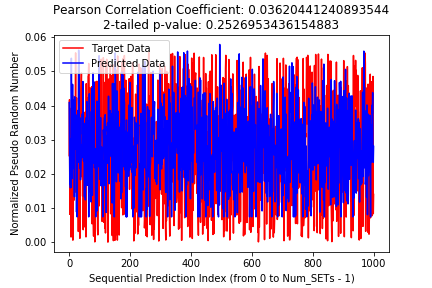
\includegraphics[width=0.4\linewidth]{./Images/Park_Miller_Reg.png}
\label{fig:PM_A}}
\qquad
\subfloat[Subfigure 2 list of figures text][Training Loss Plot]{
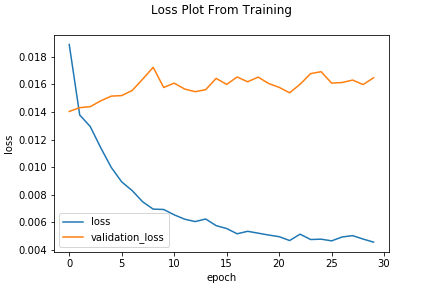
\includegraphics[width=0.4\linewidth]{./Images/Park_Miller_Loss.png}
\label{fig:PM_B}}
\caption{Park Miller Results}
\label{fig:PM}
\end{figure}

Referencing Figure~\ref{fig:PM}, our predictive model did not do well; representing about 3.6% of the variability in the data from the Park Miller PRNG. Note that with a 2-tailed p-value of 0.25, there is an indication of weak evidence for a strong model, so we can not be conclusive. We believe that increasing the quantity of training data would aide in making this a stronger model with a higher correlation coefficient and lower p-value, in addition to more training time.

\begin{figure}[H]
\centering
\subfloat[Subfigure 1 list of figures text][Testing Regression Plot]{
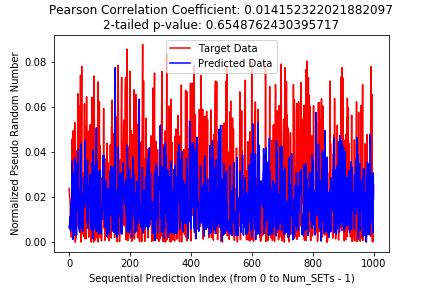
\includegraphics[width=0.4\linewidth]{./Images/Twister_Reg.png}
\label{fig:MT_A}}
\qquad
\subfloat[Subfigure 2 list of figures text][Training Loss Plot]{
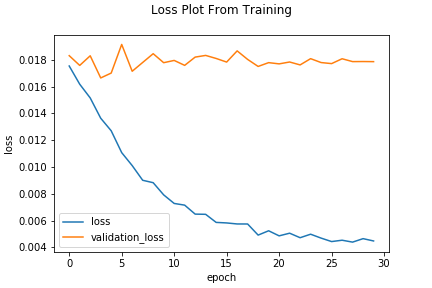
\includegraphics[width=0.4\linewidth]{./Images/Twister_Loss.png}
\label{fig:MT_B}}
\caption{Mersenne Twister Results}
\label{fig:MT}
\end{figure}

Referencing Figure~\ref{fig:MT}, our predictive model did not do well; representing about 1.4% of the variability in the data from the Mersenne Twister PRNG. Note that with a 2-tailed p-value of 0.65, there is an indication of weak evidence for a strong model, so we can not be conclusive. We believe that increasing the quantity of training data would aide in making this a stronger model with a higher correlation coefficient and lower p-value, in addition to more training time.

\begin{figure}[H]
\centering
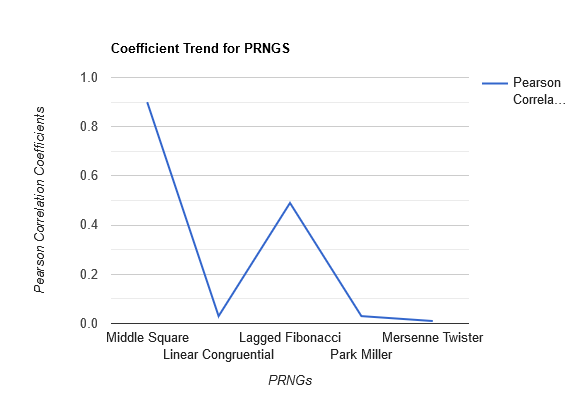
\includegraphics[width=1\linewidth]{./Images/cotrend.png}
\caption{Correlation Trend}
\label{fig:Correlation Trend}
\end{figure}
As you can see in Figure~\ref{fig:Correlation Trend}, we noticed a generally positive trend over time on the cryptographic strength of each subsequent PRNG (represented by the negative trend of the "successfulness" of each predictive model). We also can demonstrate that as we get into cryptographically stronger generation methods, our prediction success rates are noticeably less effective. Although we didn't necessarily uncover specific correlations surrounding PRNs themselves, we were able to lightly train models that, given more robust training parameters, show promise in converging a model to predict values with weak seeds. Our models also show promise due to the general progression of our loss plots, showing improvement with virtually every epoch.

% DISCUSSION SECTION
\section{Discussion}
Our main aim was to train a predictive neural net to predict the values of different PRNGs and come to generalized conclusions about the development of PRNGs with respect to time.
Throughout this research, we also ran into minor problems and noticed possible errors we could have made. Given the highly statistically precise nature of PRN generation in general, there are also areas that we could have improved on to reduce that experimental margin of error.

While developing the PRNG implementations we were having problems with the seed generation in general and recognize that a more robust seeding method could be created to eliminate the possibility for the seed to "converge" to 0. We also realize this could be a bug in the experimental code, but served nothing more than an inconvenience in the execution of the experiment. On occasion, we also experienced convergence to zero while using the middle-square PRNG implementation. On occasion the middle square implementation will converge to 0 and will cause the network training to train on convergent data, leading to faulty results when testing the predictive network. This in large has to do with the Middle-Square algorithm being known to converge given certain numbers.

Other than slight ambiguity in errors, we realize that our PRNG methods might not be perfect implementations. Some generators have tight tolerances for parameters and algorithmic behaviors. While we believe that our implementations are sound, they could be checked and improved upon by using tests of statistical randomnesses, such as the National Institute of Standards and Technology (NIST) provides. 
Different seeding methods could also provide different results, given that our seeding method was relatively linear and weak in design.

Through working on this research, we also developed an architecture that could be reused by other researchers in the future for experimentation on improved seeding methods and improved generation methods. In addition, we only ran the experiment for 30 epochs, so more computational time could be used to improve our results.

In terms of application, some practical applications for this model could be used in the future during a real-time prediction attack. If attackers were somehow able to break a strong PRNG that is used for cryptographic methods, a method like this could be used to prevent or slow down further PRN generation cycles from being compromised. 

Lastly, We encourage further work on improving the seeding methods, PRNG methods, training parameters, and model selection to produce more mathematically accurate and robust results.

.. code:: ipython3

    % REFERENCES
    % THIS IS CREATED AUTOMATICALLY
    \bibliographystyle{IEEEtran}
    \bibliography{References} % change if another name is used for References file

\end{document}
